\documentclass[../main.tex]{subfiles}
\begin{document}
\mainchapter{集合論}
\nocite{saito-kiso}

直感的自然数

\begin{figure}
    \centering
    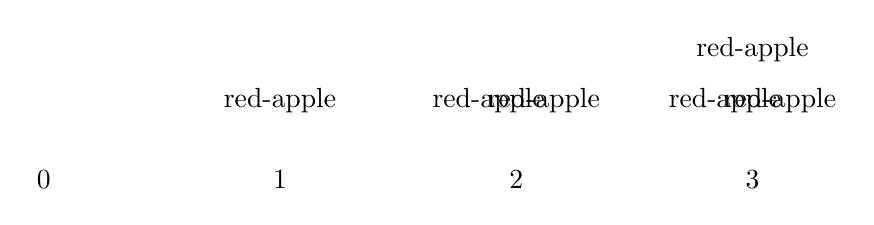
\begin{tikzpicture}
        \node at (-2, 0) {\emoji{red-apple}};

        \node at (0.65, 0) {\emoji{red-apple}};
        \node at (1.35, 0) {\emoji{red-apple}};

        \node at (3.65, 0) {\emoji{red-apple}};
        \node at (4.35, 0) {\emoji{red-apple}};
        \node at (4, 0.65) {\emoji{red-apple}};

        \node at (-5, -1) {\(0\)};
        \node at (-2, -1) {\(1\)};

        \node at (1, -1) {\(2\)};
        \node at (4, -1) {\(3\)};
    \end{tikzpicture}
    \caption{直感的自然数.}
\end{figure}


\begin{itemize}
    \item 1階の言語
        \begin{itemize}
            \item 論理記号
            \item 非論理記号\footnote{a}
                \begin{itemize}
                    \item a
                \end{itemize}
        \end{itemize}
    \item 論理の公理
        \begin{itemize}
            \item a
        \end{itemize}
    \item 集合論の公理
\end{itemize}

\begin{thmbox}
\begin{axiom}[(\ltjruby{対}{つい}の公理)]
\axiomlabel{axiom-of-paring}
\begin{align}
    \forall x \forall y \exists z \forall w (w \in z \leftrightarrow w \in x \lor w = y)
\end{align}
\end{axiom}
\end{thmbox}

これは集合\(x, y\)について\(x, y\)のみを元としてもつ集合が存在するということを述べている.
外延性公理によりこのような集合は\(1\)つだけであるから,それを\(\{x, y\}\)のように書く.
これを\(x\)と\(y\)の\keyword{非順序対}(unordered pair)という.
集合\(a\)について\(\{a, a\}\)を\keyword{\(1\)元集合}(singleton)といい\(\{a\}\)で表す.

\begin{thmbox}
\begin{definition}
集合\(a, b\)に対し,\(\{\{a\}, \{a, b\}\}\)を\(a\)と\(b\)の\keyword{順序\ltjruby{対}{つい}}(ordered pair)といい,\(\tuple{a, b}\)と表す.
\end{definition}
\end{thmbox}

\begin{proposition}
\begin{align*}
    \tuple{a, b} = \tuple{a', b'} \leftrightarrow a = a' \land b = b'
\end{align*}
\end{proposition}

\begin{proof} (\(\leftarrow\)) 明らか.

\noindent (\(\rightarrow\))
\(\{a\} \in \{\{a\}, \{a', b'\}\} \subseteq \{\{a'\}, \{a', b'\}\}\)である.
したがって\(\{a\} = \{a'\}\)または\(\{a\} = \{a', b'\}\)となる.
\end{proof}

\begin{thmbox}
\begin{proposition}
\(a, b\)が集合であるとき,\(a\)の元\(x\)と\(b\)の元\(y\)の順序対\(\tuple{x, y}\)全部集めたものは集合である.
\end{proposition}
\end{thmbox}

\end{document}
